\section{Sériové převodníky DA}
- základní zapojení a funkce, využití kapacitorů v síti, příklady využití

\subsection{Základní zapojení a funkce}
Sériové převodníky DA zaujímají zvláštní pozici mezi převodníky, v integrované podobě se prakticky nevyrábějí. Ve srovnání s paralelním převodníkem obsahuje pouze tři přesné analogové obvody, analogovou sčítačku, analogovou děličku a analogovou paměť.
\begin{figure}[h]
   \begin{center}
     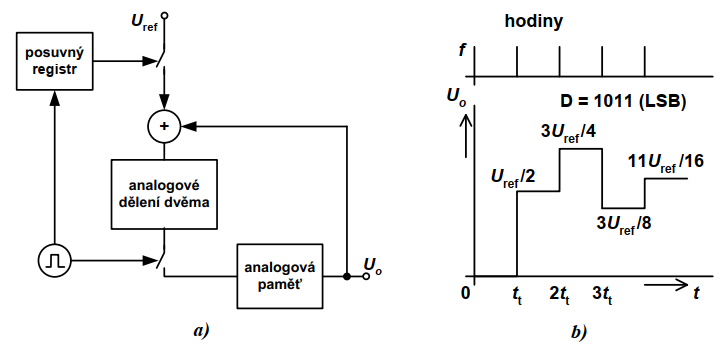
\includegraphics[scale=0.6]{images/DAser.png}
   \end{center}
   \caption{Zapojení sériového DAC}
\end{figure}

Pracují na principu postupného řízeného kvantování referenčního napětí číslicovým
signálem a sčítání váhových kvant jednotlivých bitů číslicového signálu. Sériový číslicový signál D\textsubscript{S} řídí horní spínač, který při D\textsubscript{S} = 1 připojuje kladné referenční napětí U\textsubscript{ref} do analogové sčítačky. Ve sčítačce se toto napětí sčítá s napětím u\textsubscript{k-1}, jež je udržováno na výstupu analogové paměti jako výsledek předchozího taktu převodu T\textsubscript{k-1}. Součet napětí se dělí dvěma a uloží opět do analogové paměti. Vstupní n-bitové číslo se tedy převede na analogový signál postupně, a to celkem v n taktech. Převod začíná od bitu s nejnižší vahou.

\subsection{Využití kapacitorů v síti, příklady využití}
\subsubsection{Sériový DAC s vybíjením kapacitoru}
Využívá exponenciální závislosti mezi impulzy v sériově vyjádřeném dvojkovém slově a exponenciálním tvarem vybíjecí křivky kapacitoru. Podle zjednodušeného schématu je kapacitor během první poloviny periody T/2 nabíjen ze zdroje konstantního proudu IC, pokud je však hodnota převáděného bitu rovna 1.

Protože kapacita C i proud IC jsou konstantní, bude také konstantní náboj dodaný do kapacitoru:
\begin{equation}
Q=I_{C}*\frac{T}{2}
\end{equation}
V průběhu doby T/2 napětí na kapacitoru lineárně narůstá a dosáhne hodnoty
\begin{equation}
U_{ref}=\frac{I_{C}}{C}*\frac{T}{2}
\end{equation}

\begin{figure}[h]
   \begin{center}
     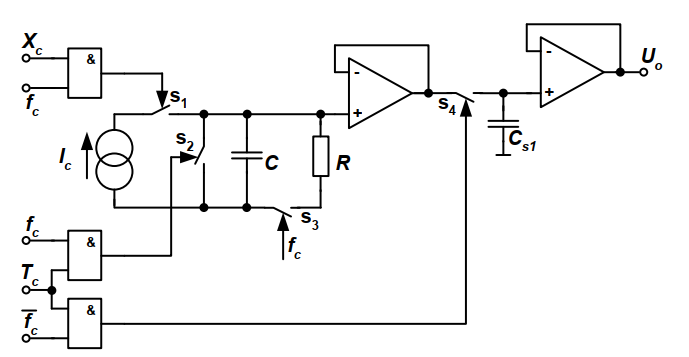
\includegraphics[scale=0.6]{images/DACC.png}
   \end{center}
   \caption{Sériový DAC s vybíjením kapacitoru}
\end{figure}

\begin{figure}[h]
   \begin{center}
     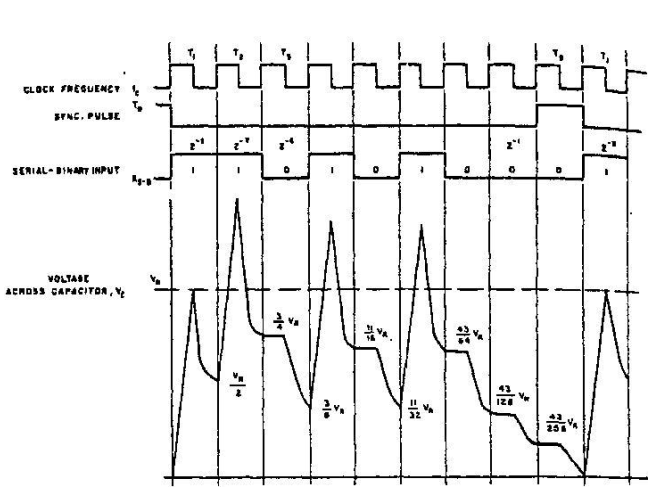
\includegraphics[scale=0.6]{images/DAgraf.png}
   \end{center}
   \caption{Příklad převodu dvojkového čísla 00101011}
\end{figure}
\newpage
\subsubsection{Sériový převodník s analogovými vzorkovači}
Sériový převodník s analogovými vzorkovači využívá rovněž metodu dělení napětí dvěma v jednotlivých taktech. 
\begin{figure}[h]
   \begin{center}
     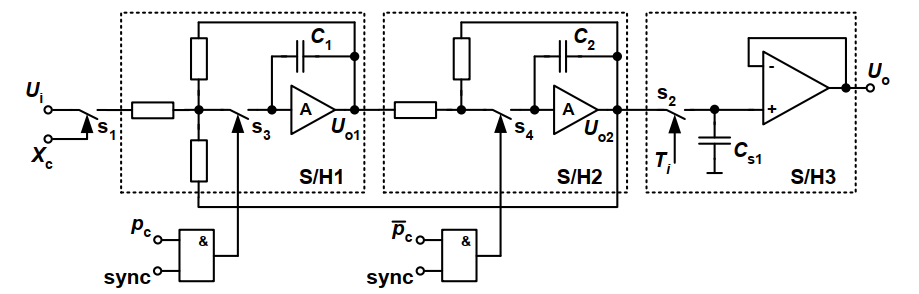
\includegraphics[scale=0.6]{images/DA2.png}
   \end{center}
   \caption{Sériový převodník s analogovými vzorkovači}
\end{figure}
Činnost každého vzorkovače může být rozčleněna do dvou fází – vzorkování a pamatování. Při sepnutých spínačích s\textsubscript{1} a s\textsubscript{3} bude vzorkovač S/H1 vzorkovat a jeho výstupní napětí se ustálí na hodnotě (je-li přenášený bit 1):
\begin{equation}
U_{o1}=-\frac{1}{2}*(U_{ref}+U_{o2})
\end{equation}
Toto vzorkování je podmíněno koincidencí hodinových impulzů a synchronizačního signálu p\textsubscript{c}. sync (tedy vždy první polovina periody Ti až do signálu sync = 1). Ve druhé polovině periody Ti se přepne S/H1 do režimu pamatování a naopak S/H2 se sepnutím s\textsubscript{4} převede do režimu vzorkování.

Vzorkovač S/H2 má v režimu vzorkování přenos -1 a uloží do své analogové paměti napětí –U\textsubscript{o1} právě ukončené předchozí poloviny periody. Cyklickým pochodem se tak v každé periodě dělí původní napětí na polovinu. Sériovým převodem se při každé 1 na pozici bitu přičítá celé U\textsubscript{ref}.
\begin{figure}[h]
   \begin{center}
     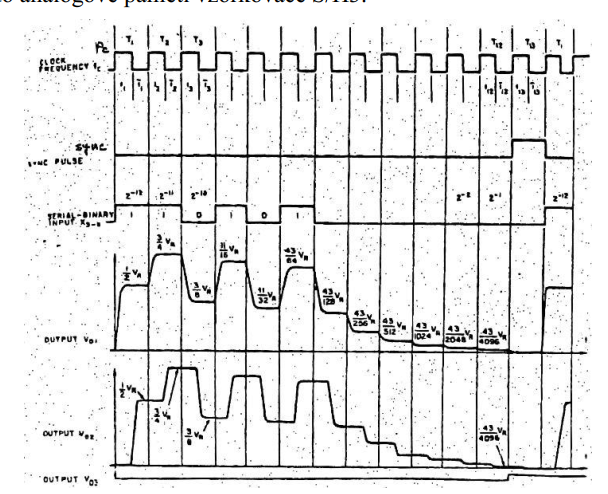
\includegraphics[scale=0.6]{images/DAgraf2.png}
   \end{center}
   \caption{Časové průběhy pro převod 12-bitového čísla na výstupní napětí}
\end{figure}

\pagebreak
\subsection{Sériový cyklický DAC s kapacitory}
Sériový cyklický DAC s kapacitory obsahuje jen dva přesné rezistory, tři paměťové kapacitory, dva OZ a napěťové spínače. Cyklický převodník je rychlejší než převodník se vzorkovači. Aktivace spínačů je symbolicky vyznačena přímou proměnnou pro aktivní 1 a invertovanou proměnnou pro aktivní 0.
\begin{figure}[h]
   \begin{center}
     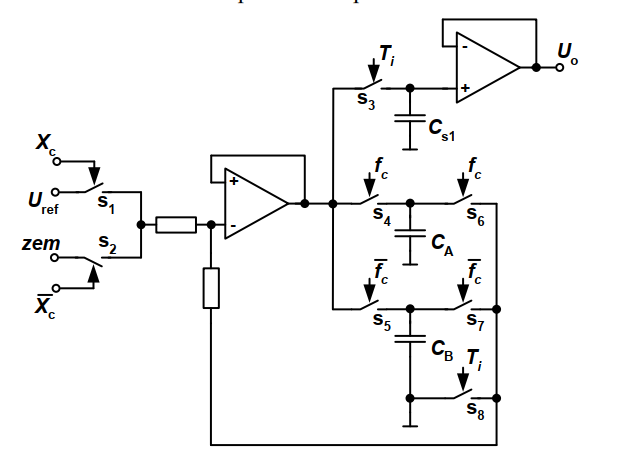
\includegraphics[scale=0.6]{images/DAser2.png}
   \end{center}
   \caption{Sériový cyklický DAC s kapacitory}
\end{figure}

Převáděné číslo je zpracováváno postupně od LSB, je-li bit = 1, spíná se s\textsubscript{1} a na vstup převodníku se přivede U\textsubscript{ref}. Pro bit s hodnotou 0 se sepnutím s2 připojí 0 V. Ostatní spínače jsou řízeny přímými nebo invertovanými signály f\textsubscript{c} (hodinové pravoúhlé impulzy), T\textsubscript{1} (identifikuje první takt) a T\textsubscript{12} (identifikuje konec převodu).

\subsection{Sériový DAC s vyrovnáním náboje}
Sériový DAC s vyrovnáním náboje využívá principu předávání (vyrovnání) náboje mezi nabitým a vybitým kapacitorem po jejich paralelním spojení. Napětí na obou spojených kapacitorech bude stejné a budou-li obě kapacity také stejné tj. C\textsubscript{1} a C\textsubscript{2}, budou stejné i oba náboje Q\textsubscript{1} = Q\textsubscript{2} a výsledné napětí bude přesně poloviční (Uref/2) proti napětí U\textsubscript{ref} původně plně nabitého kapacitoru. Vyrovnání náboje neproběhne ihned, ale s určitým zpožděním, které závisí na kapacitách C\textsubscript{1}, C\textsubscript{2} a na odporu R\textsubscript{s} sepnutého propojovacího spínače.
\begin{figure}[h]
   \begin{center}
     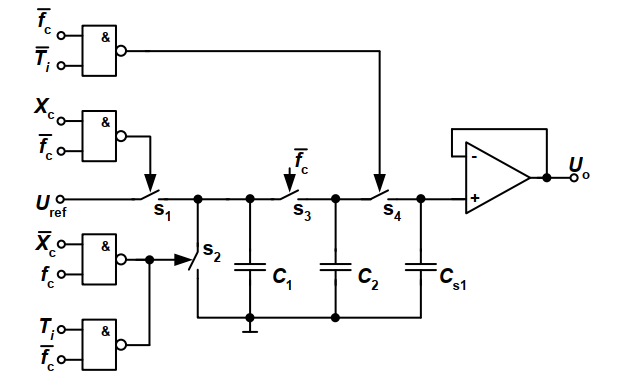
\includegraphics[scale=0.6]{images/DAvyrov.png}
   \end{center}
   \caption{Blokové zapojení sériového DAC s vyrovnáním náboje}
\end{figure}



\subsection{Nepřímé ADC}
Nepřímé převodníky DAC používají mezipřevod vstupní číslicové kombinace na jiný diskrétní signál, který je teprve převeden na výstupní analogový signál U(D). Tyto převodníky se klasifikují:
\begin{itemize}
\item vzorkováním periodických pilovitých kmitů (jedna z nejstarších metod),
\item podle druhu měronosné veličiny pomocného signálu se rozeznávají
\item nepřímé převodníky DA s mezipřevodem na poměr šířky a periody impulzů,
\item nepřímé převodníky DA s hustotou uniformních impulzů,
\item nepřímé převodníky DA s kmitočtem pravoúhlých kmitů.
\item s jiným typem mezipřevodu (magnetický modulátor, indukční dělič apod.).
\end{itemize}

V číslicově řízených kalibračních normálech napětí se užívají zejména DAC s mezi převodem na poměr šířky a periody impulzů (typicky 20-bitové převodníky). Na Obr. 96 je blokové schéma takového převodníku.
\begin{figure}[h]
   \begin{center}
     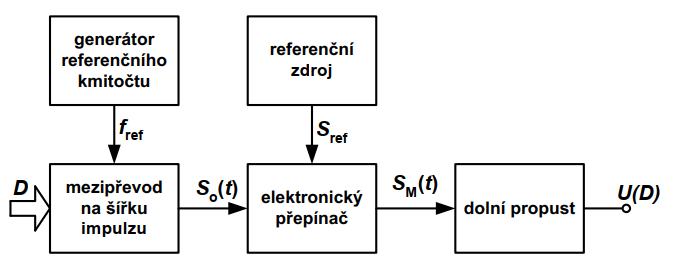
\includegraphics[scale=0.6]{images/DAneprimy.png}
   \end{center}
   \caption{Princip převodníku DAC s mezipřevodem na šířku impulzu}
\end{figure}






